\documentclass[A4]{article}
\usepackage{amsmath}
\usepackage{listingsutf8}
\lstset{basicstyle=\ttfamily, language=C} 
\usepackage[pdftex]{graphicx}
\usepackage[english]{babel} 
\usepackage[T1]{fontenc}    % font encoding;
\usepackage[utf8]{inputenc} % input encoding; can also be [cp1250] or [latin2]
\graphicspath{ {img/} }

\begin{document}
\title{Gravitational million body problem}
\author{Amadej Tratnik, Filip Zupančič}
\maketitle
\section{Problem}
Imagine n bodies in space with masses $m_i$ (i = 1, 2, ..., n). We want to calculate mutual gravitational forces and analyze dynamics of such system. 
\section{Solution}
\subsection{Logic}
Newtons equation that describes movement in the system is suitable for our problem
\[
\ddot{x} = \sum_{j \neq i} G \frac{m_j}{|x_j - x_i|^3}(x_j - x_i), \quad i = 1, . . . , n
\]
\newline
$x_i = (x_i, y_i, z_i)$ is the position mass of body with index i, G gravitational constant (can be 1). We presume masses are dotted. We will also disregard radius of objects in comparison to distances. 
\newline
Time dependence of is $n^2$. That's why we decided to implement solution in C instead of Octave. 
\newline
In the middle of the system is positioned object with big mass (black hole) with coordinates (0,0,0). Other objects have random coordinates in space around black hole. To compute distances between big mass object and bodies is used Pythagoras equation
\[
r = \sqrt{x^2 + y^2 + z^2}
\]
\newline
We use 2nd Newton's law F = ma. Circumferential speed has direction of tangent on circumference and represents derivation of route through time. 
\[
v = \frac{ds}{dt}
\]
\newline
Angular velocity is determined by derivation of angle of rotation over time.
\[
w = \frac{dl}{dt}
\]
Peripheral speed and circumferencial speed are connected with relation 
\[
v = rw
\]
Radial acceleration can be written like 
\[
a_r = w^2r = \frac{v^2}{r}
\]
With help of 2nd Newtons law we get 
\[
F_r = mw^2r = \frac{mv^2}{r}
\] 
Radial force is equal to force of gravity 
\[
F_g = mg = G\frac{Mm}{r^2} \quad => \quad \frac{mv^2}{r} = G\frac{Mm}{r^2}/r \quad => \quad v^2 = G\frac{M}{r} \quad => \quad v = \sqrt{\frac{M}{r}} 
\]
\newline
In the calculations we didn't use gravitational constant because it doesn't differ the visualization. We defined initial velocities in the directions x, y and z as 
\[
	\begin{bmatrix} 
    	-v+\frac{y}{r} \\
	v+\frac{x}{r} \\
	0
	\end{bmatrix}
\]  
\newline
To compute the forces between bodies we used the equation 
\[
\ddot{x} = \sum_{j \neq i}\frac{m_j}{|x_j - x_i|^3}(x_j - x_i), \quad i = 1, . . . , n
\]
\newline
In every iteration we compute difference between coordinates x, y, z and get 
\[
D = \sqrt{dx^2 + dy^2 + dz^2}
\]
\newline
\[
\begin{bmatrix} 
    	dx = x_i - x_j \\
	dy = y_i - y_j \\
	dz = z_i - z_j
	\end{bmatrix}
\]
\newline
Then we use 3rd Newton's law $[\vec{F_{21}} = \vec{-F_{12}}]$. This means that we add force to body on index i and substract force from the body on index j. Time dependence drops from $O(n^2)$ to $O(\frac{n^2}{2})$ .
\newline \newline
In real time program successfully computes forces and new coordinates for about 1500 bodies. Future improvements are parallel processing and processing on graphic card. 
\newline
solution.c contains functions generate-parameters() that generates initial parameters as velocities and coordinates, that are random points in space. Masses of all bodies are 1 except for the black hole that has a mass 10000000. Function compute-coordinates() computes forces between bodies and calculates new coordinates of bodies that are saved in array coordinates. Helper.h holds global parameters as arrays masses (length number of bodies), coordinates (xyz for every body) and velocities (in directions xyz).
\begin{figure}[t!]
\centering
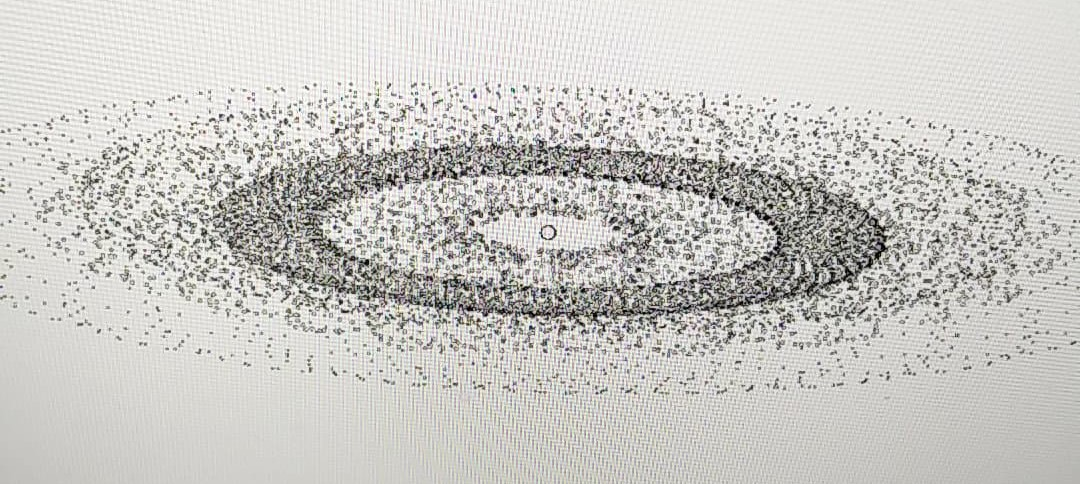
\includegraphics[width=\textwidth]{three_bodies_octave}
\caption{system of three bodies implemented in octave. It's time consuming.}
\end{figure}
\subsection{Visualization} 
Glut is a wonderful OpenGL library and it suits perfectly for our problem. Inside visualization.c is a function visualize() that initializes window and creates main loop. Function display() draws bodies in 3D space. Refresh interval is set to 15ms. Function resize() resizes window when we want to expand or minimize window on full screen. Program also reads simple input from keyboard. 
\newpage
\begin{figure}[t!]
\centering
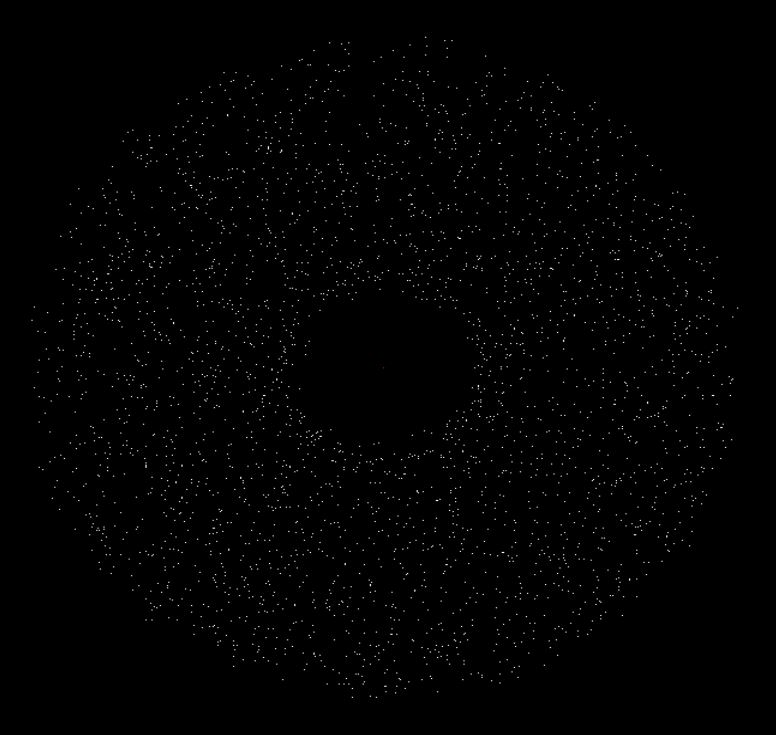
\includegraphics[width=\textwidth]{visualization}
\caption{system of three thousand bodies implemented in C.}
\end{figure}

\end{document}